% Options for packages loaded elsewhere
\PassOptionsToPackage{unicode}{hyperref}
\PassOptionsToPackage{hyphens}{url}
%
\documentclass[
]{article}
\usepackage{amsmath,amssymb}
\usepackage{lmodern}
\usepackage{ifxetex,ifluatex}
\ifnum 0\ifxetex 1\fi\ifluatex 1\fi=0 % if pdftex
  \usepackage[T1]{fontenc}
  \usepackage[utf8]{inputenc}
  \usepackage{textcomp} % provide euro and other symbols
\else % if luatex or xetex
  \usepackage{unicode-math}
  \defaultfontfeatures{Scale=MatchLowercase}
  \defaultfontfeatures[\rmfamily]{Ligatures=TeX,Scale=1}
\fi
% Use upquote if available, for straight quotes in verbatim environments
\IfFileExists{upquote.sty}{\usepackage{upquote}}{}
\IfFileExists{microtype.sty}{% use microtype if available
  \usepackage[]{microtype}
  \UseMicrotypeSet[protrusion]{basicmath} % disable protrusion for tt fonts
}{}
\makeatletter
\@ifundefined{KOMAClassName}{% if non-KOMA class
  \IfFileExists{parskip.sty}{%
    \usepackage{parskip}
  }{% else
    \setlength{\parindent}{0pt}
    \setlength{\parskip}{6pt plus 2pt minus 1pt}}
}{% if KOMA class
  \KOMAoptions{parskip=half}}
\makeatother
\usepackage{xcolor}
\IfFileExists{xurl.sty}{\usepackage{xurl}}{} % add URL line breaks if available
\IfFileExists{bookmark.sty}{\usepackage{bookmark}}{\usepackage{hyperref}}
\hypersetup{
  pdftitle={Wiring between close nodes in biological networks evolves more quickly than between distant nodes},
  pdfkeywords={network biology, interactome, network evolution, phylogenetic comparative methods, drug-drug interactions},
  hidelinks,
  pdfcreator={LaTeX via pandoc}}
\urlstyle{same} % disable monospaced font for URLs
\usepackage[margin=1in]{geometry}
\usepackage{longtable,booktabs,array}
\usepackage{calc} % for calculating minipage widths
% Correct order of tables after \paragraph or \subparagraph
\usepackage{etoolbox}
\makeatletter
\patchcmd\longtable{\par}{\if@noskipsec\mbox{}\fi\par}{}{}
\makeatother
% Allow footnotes in longtable head/foot
\IfFileExists{footnotehyper.sty}{\usepackage{footnotehyper}}{\usepackage{footnote}}
\makesavenoteenv{longtable}
\usepackage{graphicx}
\makeatletter
\def\maxwidth{\ifdim\Gin@nat@width>\linewidth\linewidth\else\Gin@nat@width\fi}
\def\maxheight{\ifdim\Gin@nat@height>\textheight\textheight\else\Gin@nat@height\fi}
\makeatother
% Scale images if necessary, so that they will not overflow the page
% margins by default, and it is still possible to overwrite the defaults
% using explicit options in \includegraphics[width, height, ...]{}
\setkeys{Gin}{width=\maxwidth,height=\maxheight,keepaspectratio}
% Set default figure placement to htbp
\makeatletter
\def\fps@figure{htbp}
\makeatother
\setlength{\emergencystretch}{3em} % prevent overfull lines
\providecommand{\tightlist}{%
  \setlength{\itemsep}{0pt}\setlength{\parskip}{0pt}}
\setcounter{secnumdepth}{-\maxdimen} % remove section numbering
\ifluatex
  \usepackage{selnolig}  % disable illegal ligatures
\fi
\newlength{\cslhangindent}
\setlength{\cslhangindent}{1.5em}
\newlength{\csllabelwidth}
\setlength{\csllabelwidth}{3em}
\newenvironment{CSLReferences}[2] % #1 hanging-ident, #2 entry spacing
 {% don't indent paragraphs
  \setlength{\parindent}{0pt}
  % turn on hanging indent if param 1 is 1
  \ifodd #1 \everypar{\setlength{\hangindent}{\cslhangindent}}\ignorespaces\fi
  % set entry spacing
  \ifnum #2 > 0
  \setlength{\parskip}{#2\baselineskip}
  \fi
 }%
 {}
\usepackage{calc}
\newcommand{\CSLBlock}[1]{#1\hfill\break}
\newcommand{\CSLLeftMargin}[1]{\parbox[t]{\csllabelwidth}{#1}}
\newcommand{\CSLRightInline}[1]{\parbox[t]{\linewidth - \csllabelwidth}{#1}\break}
\newcommand{\CSLIndent}[1]{\hspace{\cslhangindent}#1}

\title{Wiring between close nodes in biological networks evolves more quickly than between distant nodes}
\author{true \and true}
\date{}

\begin{document}
\maketitle
\begin{abstract}
Lorem ipsum dolor sit amet, consectetur adipiscing elit. Curabitur eget porta erat. Morbi consectetur est vel gravida pretium. Suspendisse ut dui eu ante cursus gravida non sed sem. Nullam sapien tellus, commodo id velit id, eleifend volutpat quam. Phasellus mauris velit, dapibus finibus elementum vel, pulvinar non tellus. Nunc pellentesque pretium diam, quis maximus dolor faucibus id. Nunc convallis sodales ante, ut ullamcorper est egestas vitae. Nam sit amet enim ultrices, ultrices elit pulvinar, volutpat risus.
\end{abstract}

{
\setcounter{tocdepth}{2}
\tableofcontents
}
\hypertarget{introduction}{%
\section{Introduction}\label{introduction}}

Biological networks are representations of molecular interactions in the cell. These networks are constructed by collecting biochemical and genetic interactions from different kinds of biological entities, an approach that has improved drastically in the last decades with the advent of modern high-throughput methods. However, there are still many limitations for the gathering and analysis of biological networks, specifically for modelling network evolution across and within species. This is because many biological networks have poor quality or are incomplete, and because the number of organisms for which network data is available is still very limited (Jin et al. 2013; Cusick et al. 2005; Ghadie, Coulombe-Huntington, and Xia 2018). Despite these limitations, many advances have been made in characterizing static networks, and in developing a theoretical framework for studying their evolution across species.

Biological networks evolve as nodes and edges are added or lost in the network. This can be the result of different processes affecting network content, such as gene duplication, gene loss, pseudogenization, HGT or WGD (Wagner 2003; Cork and Purugganan 2004), or a result of processes affecting quantitative properties, including non-synonymous substitutions in the nodes affecting their function (e.g.~mutations affecting the binding of ligands, protein domains or DNA motifs may result in changes in metabolic processes, signaling pathways or gene expression regulation, among others) (Jensen 1976; Ghadie, Coulombe-Huntington, and Xia 2018). These evolutionary events remove old connections and generate new ones, in a process that may be random. However, we also know that not all motifs are equally abundant in biological networks (Picard et al. 2008). This may be the result of natural selection removing deleterious connections and favoring advantageous ones. In addition to this, rewiring rates vary depending on several factors. For example, the type of network may have an effect in rewiring rates, since some networks networks such as gene regulatory networks tend to rewire at faster rates than more constrained networks such as metabolic networks (Shou et al. 2011).

Rewiring rates also vary within networks, such as between different network modules and between nodes depending on their importance for the cell's survival and reproduction, and the essentiality of a node or module may be a constraining factor for network evolution. Previous studies have shown an inverse relationship between highly connected proteins and their rate of substitution (Fraser et al. 2002), possibly due to strong purifying selection acting on the interfacial sites of interacting proteins (Zotenko et al. 2008).

Despite these advances at studying the connections of individual nodes and global network rewiring rates, the rate at which quantitative differences between networks accumulate as a function of species divergence remains relatively unexplored. In particular, it is unknown whether evolutionary rates of inter-node connectivity are correlated with inter-node network measures, such as the minimum path length or average node degree between nodes.

In this paper, we use drug-drug interactions (DDIs as a quantitative proxy measurement of inter-node connectivity, since it has been shown that DDIs are partially dependent on the underlying network topology between targets (Lehar et al. 2007; Yeh et al. 2009). Drug-drug interactions (DDIs) occur when the effect of two or more drugs is significantly stronger or weaker than their expected combined effect, respectively named synergies and antagonisms (Cowen and Steinbach 2008). DDIs are used in the development of novel pharmacological treatments with higher efficiencies at lower doses with the aim of reducing the evolution of drug resistance (Cowen and Steinbach 2008). The reasons why a DDI occurs are varied, but it has been shown that a DDI can occur as a result of factors such as (1) the topology of the underlying network between drug targets, (2) the essentiality of the metabolites blocked by the perturbation, and the inhibition efficiency of the drug on the drug target (Yeh et al. 2009). For example, synergies can occur if drugs act on parallel pathways, where the individual effect of each drug is small and an alternative pathway can compensate for the effect of a single drug (Yeh et al. 2009). Alternatively, antagonistic interactions can occur mainly in two different ways: by causing a partial loss of function in two parallel pathways of an essential product, or as a result of drugs acting sequentially along the same pathway (Yeh et al. 2009). This relation between DDIs and network topology has been further explored using experiments and metabolic flux simulations in yeast, suggesting that specific combinations of perturbations in the network result in different quantifiable interaction scores (Lehar et al. 2007). More recently, it has been shown that most synergistic interactions are the result of drugs targeting the same cellular process, while antagonistic interactions are the result of drugs targeting different processes (Brochado et al. 2018).

Only a few studies have explored interspecific variation of DDIs (Spitzer et al. 2011; Robbins et al. 2015; Brochado et al. 2018), but they have shown that DDI scores could be scalable to include higher numbers of species and strains, allowing for the evaluation of network evolution hypotheses within and between species. A high throughput study of DDIs in gram-negative bacteria has shown that antagonistic interactions are more common, and are almost exclusively detected on drugs that target different cellular processes, while synergies are more conserved across species, and they are more frequent in drugs that target the same process (Brochado et al. 2018). In that study, 70\% of the DDIs detected were species-specific, while 20\% were strain-specific.

Given these previous findings, we had two related questions. First, do DDI scores diverge as a function of species divergence, consistent with neutral processes acting on the underlying network structure? Or is there substantial constraint on some DDI scores, consistent with evolutionary constraint on the drug targets, their connectivity, and the drugs' mode of action?

Second, do synergistic interactions evolve at a slower rate than other types of drug interactions, and antagonistic interactions evolve at a faster rate? These differences in rates would be a result of synergistic interactions taking place in local neighborhoods of nodes, while antagonistic interactions act on distant network neighborhoods, which appear to evolve more slowly because of greater network redundancy between distant nodes. Indeed, if we were to map DDIs to protein targets (when known), are the drug targets of synergistic drug interactions closer in the network than additive and antagonistic interactions? And, more generally, are more closely connected nodes subject to higher rates of evolution than more distantly related nodes?

To address these questions, we used the most complete available dataset of species specific and strain specific DDIs (Brochado et al. 2018). We modelled these DDIs under a phylogenetic comparative framework and applied a multivariate brownian motion model to estimate the evolutionary rate of interaction scores for different clusters of DDIs in six strains (three species) of gram-negative bacteria. We also mapped DDIs to their putative protein targets to evaluate them in known biological networks. We show that DDIs can be used as an effective proxy to evaluate macroevolutionary implications and the role of network evolution in interspecific variation.

\hypertarget{methods}{%
\section{Methods}\label{methods}}

We obtained DDI scores from a previous study (Brochado et al. 2018) that assessed almost 3000 combinations of 79 different compounds on six strains of three species of gram-negative bacteria (pae: \emph{P. aeruginosa PAO1}, pau: \emph{P. aeruginosa UCBPP-PA14}, stm: \emph{S. enterica subsp. enterica serovar Typhimurium LT2}, seo: \emph{S. enterica subsp. enterica serovar Typhimurium 14028S}, ecr: \emph{E. coli O8 IAI1 (commensal)}, ebw: \emph{E. coli K-12 BW2952)}. In particular, we used their following datasets, tables ED09C for modelling DDI evolution, and Sup. Tables 1 and 2 to compare different categories of drugs. We constructed phylogenetic trees of the six strains using PhySpeTree to obtain estimate branch lengths (Fang et al. 2019). We used concatenated alignments of 35 highly conserved protein sequences (HCP), and specified the iqtree pipeline within PhySpeTree.

\hypertarget{clustering-ddi-using-tsne.}{%
\subsubsection{Clustering DDI using tSNE.}\label{clustering-ddi-using-tsne.}}

To reduce the dimensionality of the DDI data, we classified DDIs into clusters using tSNE in the R packages bigMap (Garriga and Bartumeus 2018) and bigmemory (Kane, Emerson, and Weston 2013), with the following parameters (threads=80, layers=80, rounds=9). Dimensionality reduction was performed to increase robustness of rate estimators given the small number of species used. Our tSNE analysis was performed for a range of perplexity values between 50 and 2120. DDIs were clustered by similarity across strains, treating each strain as a dimension, thus DDIs that are closer to each other across strains would cluster together under tSNE. The clustering output was visualized and evaluated based on the stability and plateauing of cost and effect size curves. We obtained stable solutions between 700 and 900 perplexity values with this approach. In order to have a more accurate prediction of perplexity, we repeated the previous approach on this smaller range of values. In both cases, the pakde algorithm was applied with perplexity of 1/3 the respective tSNE perplexity. In the range explored, we obtained two optimal solutions at perplexities of 706 and 825, with 13 and 4 clusters respectively. In order to find what solution was optimal, we tested for modularity in the data using the function phylo.modularity within the package geomorph (Adams et al. 2016), which indicated that a perplexity of 706 results in more modular clustering. Thus, we fitted a multivariate brownian motion model to the most modular clustering pattern and calculated the evolutionary rates per cluster using compare.multi.evol.rates, within the package geomorph (Adams et al. 2016). These cluster rates were used as approximations for DDI evolutionary rates, for the DDIs in each of the clusters.

\hypertarget{identification-of-drug-targets-and-their-biological-networks.}{%
\subsubsection{Identification of drug targets and their biological networks.}\label{identification-of-drug-targets-and-their-biological-networks.}}

Each drug was identified to a unique Pubchem and CHEMBL IDs using webchem (Szöcs et al. 2020), which were used to retrieve their mode of action from IUPHAR (Armstrong et al. 2020). Similarly, we compared our targets to a previously published dataset on drugs and drug targets (Santos et al. 2017). We identified unique Uniprot IDs and KO IDs for each target protein, and converted these IDs into \emph{E. coli} Uniprot IDs using KEGG (Kanehisa and Goto 2000). We didn't include in the analysis drugs whose mode of action was unknown, or that had non-protein molecules as targets, such as small molecules, RNA or DNA.

Biological networks of \emph{E. coli} were downloaded from EcoliNet (Kim et al. 2015). EcoliNet networks are constructed using inferred links based on different factors such as: co-citation (CC), co-expression (CX), co-occurrence of protein domains (DC), similar genomic context of bacterial orthologs (GN), high-throughput protein-protein interactions (HC), small/medium-scale protein-protein interactions (LC), and similarity of phylogenetic profiles (PG).

\hypertarget{calculating-inter-node-network-metrics.}{%
\subsubsection{Calculating inter-node network metrics.}\label{calculating-inter-node-network-metrics.}}

For each of the networks we calculated the average path length, and node degree distributions. In addition, the minimum distance between each of the nodes in the network was calculated, as well as the node degree (number of connection per node), and the k-edge connectivity between each pair of nodes (i.e.~the minimum number of edges that can be remove to disconnect the nodes). We used the R package igraph (Csardi and Nepusz 2006) to calculate these values in each one of the biological networks and for each node or pair of nodes. We also generated an adjacency matrix, which contains information on whether two nodes are connected directly by an edge or not. In addition, we used k-edge connectivity as a proxy for connectedness between proteins (i.e.~a pair with k-edge connectivity equal to zero is disconnected, proteins with k-edge connectivities different than zero are connected). Connectedness is used due to the limitations of adjacency in describing the overall connection between nodes.

Code availability. The code used for data analysis is available from \url{https://github.com/phylogenomic/ch3-netbio}

\hypertarget{results}{%
\section{Results}\label{results}}

\hypertarget{ddi-divergence-between-the-strains-increases-as-a-function-of-species-divergence.}{%
\subsubsection{DDI divergence between the strains increases as a function of species divergence.}\label{ddi-divergence-between-the-strains-increases-as-a-function-of-species-divergence.}}

We also examined variance among six strains in their drug drug interaction (DDI) scores using PCA, and found that Pseudomonas and non-Pseudomonas strains differentiate well along the first principal component axis, which explains 47\% of the variance (\textbf{Fig. \ref{fig:fig1}C}). The second axis distinguishes between \emph{E. coli} and \emph{Salmonella} strains and explains 22\% of the variance. Strains of the same species group closely together in the PCA space, indicating that they share similar global DDI responses.

We then performed hierarchical clustering of the six strains based on their DDI scores (``Strains'' in \textbf{Fig. \ref{fig:fig1}B}). We also generated a phylogenetic tree based on highly conserved proteins (\textbf{Fig. \ref{fig:fig1}A}). In both analyses, the Enterobacteriaceae species (\emph{E. coli} and \emph{S. enterica}) are distantly related to \emph{Pseudomonas}. The clustering based on DDIs yielded the same tree topology as the gene-based phylogeny. To test whether DDI scores (``chemical distance'') diverge as a function of species divergence, we used linear and logarithmic regressions, which measured the amount of DDI variation explained by sequence divergence (Manhattan distance on the phylogeny). We obtained an R\textsuperscript{2} value of 0.406 for logarithmic regression (\textbf{Fig. \ref{fig:fig1}D}), and an R2 of 0.733 for linear regression, after a log transformation of the phylogenetic distance (\textbf{Fig. \ref{fig:fig1}E}). These results suggest that DDIs, and their underlying network basis, diverge as a function of sequence divergence. Chemical divergence plateaus at higher phylogenetic divergence values; this type of saturation has been previously reported in models of network evolution for rewiring rates across species (Shou et al. 2011).

An examination of hierarchical clustering across DDIs reveals DDI clusters that are conserved, or vary similarly, across strains (``Drug-Drug Interactions'' in \textbf{Fig. \ref{fig:fig1}B}). An example of this can be seen at the bottom of \textbf{Fig. \ref{fig:fig1}B}, where DDIs that are highly synergistic in all species (shown in blue) group together in the bottom rows. We also categorized DDIs by whether the two drugs belong to the same drug category, target the same cellular process, or have the same use. We observed that highly synergistic DDI across all species tend to occur when both drugs belong to the same chemical category and target the same cellular process, consistent with previous reports (Brochado et al. 2018).

\begin{figure}
\includegraphics[width=1\linewidth]{Fig1} \caption{Drug-drug interaction (DDI) chemical distance scales with phylogenetic distance. **A.** Maximum likelihood phylogeny of six strains based on highly conserved proteins. **B.** Heatmap of DDI by strain data. Hierarchical clustering based on euclidean distances was performed for strains (columns) and DDIS (rows). **C.** Phylomorphospace plot combining a PCA of the DDI data with the phylogeny; principal components 1 and 2 are shown.  **D.** DDI euclidean distances between strains scale as a function of phylogenetic distance. This relationship saturates at large phylogenetic distances. Intraspecific comparisons (in blue) have the lowest amount of sequence and chemical divergence, while comparisons with *Pseudomonas* are the most distant in terms of sequence and chemical divergence. **E.** Same comparison shown as a linear relationship when phylogenetic distance is log transformed.}\label{fig:fig1}
\end{figure}

\hypertarget{synergistic-interactions-have-the-shortest-average-distance-between-targets-followed-by-additive-and-antagonistic-interactions.}{%
\subsubsection{Synergistic interactions have the shortest average distance between targets, followed by additive and antagonistic interactions.}\label{synergistic-interactions-have-the-shortest-average-distance-between-targets-followed-by-additive-and-antagonistic-interactions.}}

Out of the 79 compounds analyzed, we were able to identify protein targets for 23 compounds using a database developed by Santos et al.~(2017). These compounds had a total of 26 target proteins as identified by their unique protein IDs in \emph{E. coli}, where the most common target category was bacterial penicillin binding protein, a group involved in the biosynthesis of bacterial cell walls. Other target categories mapped include ribosomal, DNA polymerase, topoisomerase, thymidylate synthase and mitochondrial glycerol-3-phosphate (\textbf{Sup. Table 1}). \textbf{Describe only PPI network} (\textbf{Fig. \ref{fig:fig2}}).

\begin{figure}
  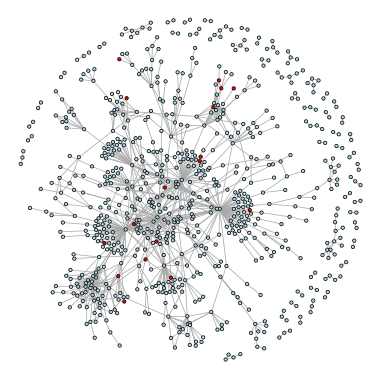
\includegraphics[width=1\linewidth]{Fig2} \caption{Graphical representation of the PPI network from *E. coli*, as determined by small and medium scale experiments [@Kim2015]. Each node represents a unique Uniprot ID and red nodes are target proteins identified as participating in DDIs in our analysisThis network contains 767 nodes with an average path length of 4.9.}\label{fig:fig2}
  \end{figure}

We measured the length of minimum distance paths between all targets across all networks, and found that synergistic interactions have the shortest average distance, followed by additive interactions, and antagonisms. These results were found in all biological networks under study except two, co-expression (CX) and high-throughput protein-protein interaction (HT) networks (\textbf{Fig. \ref{fig:fig3}}). This result is consistent with our previous expectations, given that synergistic interactions tend to be more common between drugs that target the same cellular process, and thus should be closer to each other in biological networks. In addition to this, we repeated this analysis comparing interaction type with two other metrics, k-edge connectivity (\textbf{Sup. Fig. 1}) and average node degree (\textbf{Sup. Fig. 2}). We didn't find a consistent pattern that showed clear differences between synergistic, additive and antagonistic interactions across all networks, suggesting that there may not be clear differences between different types of drug interactions for connectivity or node degree between targets.

\begin{figure}
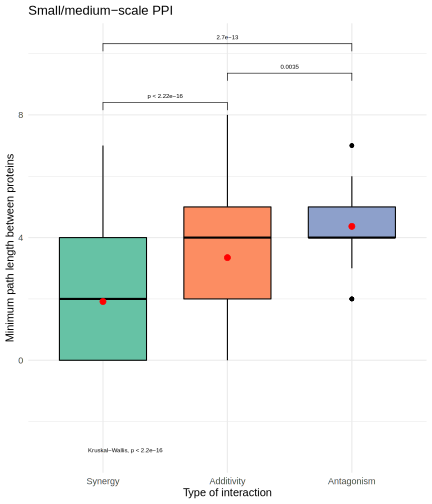
\includegraphics[width=1\linewidth]{Fig3} \caption{Differences in minimum path length between targets for different types of drug interactions in E. coli for different biological networks. Synergistic interactions have a lower average than additive interactions, followed by antagonisms. This pattern is detected in all networks except the co-expression and the high-throughput protein-protein interaction network.}\label{fig:fig3}
\end{figure}

\hypertarget{synergistic-interactions-have-faster-evolutionary-rates-than-additive-and-antagonistic-interactions.}{%
\subsubsection{Synergistic interactions have faster evolutionary rates than additive and antagonistic interactions.}\label{synergistic-interactions-have-faster-evolutionary-rates-than-additive-and-antagonistic-interactions.}}

We sought to estimate the evolutionary rate of DDI change. However, there is low power with only six tips to estimate rate shifts for any individual DDI. Instead, we used tSNE to detect clusters of DDIs that behave similarly across species, allowing for increased power within each cluster. From this analysis we obtained two different optimal solutions for each of the perplexity ranges explored, one clustering solution with perplexity 706 for the large range analysis (\textbf{Sup. Document 1}) and another solution with perplexity 825 for the small range analysis (\textbf{Sup. Document 2}). These yielded 13 (\textbf{Fig. \ref{fig:fig4}A}) and 4 (\textbf{Fig. \ref{fig:fig4}B}) distinct DDI clusters, respectively. We didn't detect any clear differentiation among clusters by drug category or cellular processes targeted by each drug (\textbf{See tSNEplots}). We conducted 1000 random permutations of the phylo modularity test to determine the optimal clustering solution out of the two obtained. The test supported the 13 cluster solution as the one with the strongest modular signal (p value=0.001, effect size=-26.3594, CR=0.9231, CI= \{0.8643,1.0121\}) over the 4 clusters (p value=0.001, effect size=-13.9241, CR=0.985, CI=\{0.9544,1.0049\}) (Adams et al.~2016), and we therefore use that going forward.

We next calculated the evolutionary rate of each of the 13 clusters by estimating the sigma parameter for each of the clusters using a multivariate Brownian motion model. We detected significant differences between clusters (observed rate ratio 12.9955, p value=0.003). In particular, we noticed that clusters 13 and 2 had very high evolutionary rates of 57.3 and 27.6 respectively, while all the other clusters had rates ranging from 4.4 to 24.2.

We detected significant differences between types of interactions for DDI evolutionary rates, where synergistic interactions have faster evolutionary rates than additive and antagonistic interactions. This pattern was consistently found across all types of biological networks (\textbf{Fig. \ref{fig:fig5}}).

\hypertarget{wiring-between-close-nodes-in-biological-networks-evolves-more-quickly-than-between-distant-nodes.}{%
\subsubsection{Wiring between close nodes in biological networks evolves more quickly than between distant nodes.}\label{wiring-between-close-nodes-in-biological-networks-evolves-more-quickly-than-between-distant-nodes.}}

Given the relationship between interaction type and minimum distance shown earlier, we also tested whether evolutionary rates are affected by minimum distance between targets. In the small-medium scale protein-protein interaction network (\textbf{Fig. \ref{fig:fig6}}) There is a decline in evolutionary rates as a function of minimum distance between targets. We interpret this to mean that wiring between close nodes in biological networks evolves more quickly than between distant nodes.
Other networks such as co-citation (CC),co-functional gene-pairs (GO-BP), or phylogenomic profiles (PG) show a sharp decline in rates as a function of distance followed by a rebounce in the rate when distance was greater than about 4 or 6 steps respectively (\textbf{see supplement}).

\begin{figure}
\includegraphics[width=1\linewidth]{Fig4} \caption{A. Visualization of tSNE results. Top left: tSNE plot at perplexity 706 yielded 13 unique clusters. Top right: WTT plot showing cluster density and boundaries for perplexity 706. Bottom left: tSNE plot at perplexity 825 yielded 4 clusters. Bottom right. WTT plot showing cluster density and boundaries for perplexity 825. B. Multivariate evolutionary rates for each of the tSNE clusters at perplexity 825 (x axis ordered by rate)}\label{fig:fig4}
\end{figure}

\begin{figure}
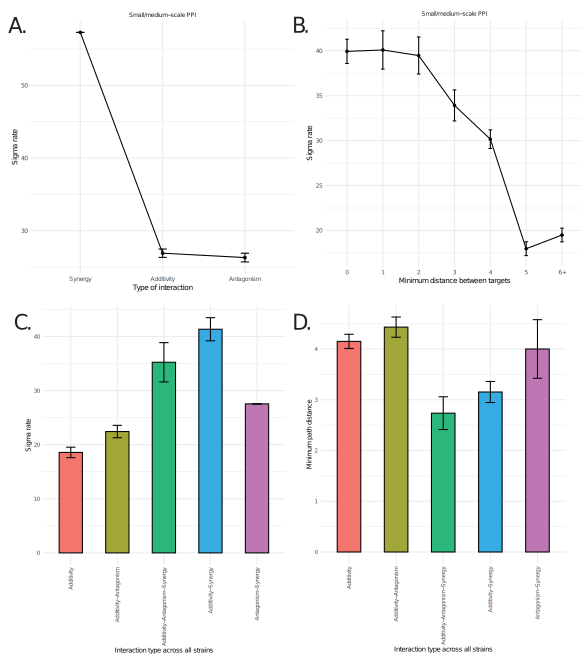
\includegraphics[width=1\linewidth]{Fig5} \caption{ Evolutionary rate as a function of type of interaction for the small/medium scale PPI network. Synergistic interactions have higher evolutionary rates than additive and antagonistic interactions across all network types.}\label{fig:fig5}
\end{figure}

\begin{figure}
\includegraphics[width=1\linewidth]{Fig6} \caption{Evolutionary rate as a function of  minimum distance between targets. Wiring between close nodes in biological networks evolves more quickly than between distant nodes.}\label{fig:fig6}
\end{figure}

\hypertarget{other-factors-that-contribute-to-variation-in-evolutionary-rates.}{%
\subsubsection{Other factors that contribute to variation in evolutionary rates.}\label{other-factors-that-contribute-to-variation-in-evolutionary-rates.}}

We also wanted to evaluate the role that other network parameters play in differences in evolutionary rates for different DDIs, such as connectedness (whether two nodes are connected through a path), adjacency (whether two nodes are directly linked), k-edge connectivity (i.e.~minimum number of connections that have to be broken to disconnect two nodes), and average node degree (the average number of connections in a pair of target proteins). We found that the effect of connectedness and adjacency vary widely by network type. In the case of connectedness, connected targets had a slower evolutionary rates than disconnected in 10/11 networks (\textbf{Sup. Fig. 3}). In contrast, we found that adjacent nodes tend to have higher evolutionary rates than non-adjacent nodes in 7/10 types of networks (\textbf{Sup. Fig. 4}). These opposite results can be made compatible if we consider that connectedness was defined as k-edge connectivity different than 0, while adjacency refers the presence of a direct link between targets. Furthermore, differences in evolutionary rates at finer scales, such as modeling evolutionary rates by k-edge connectivity or average node degree between protein targets yielded results that vary widely depending on the type of network under consideration. In some networks (EcoCyc/GO-BP,EN, GO-BP, HT PPI) it appears that the most connected nodes have higher evolutionary rates, while intermediate and low k-edge connected nodes have a variable range of evolutionary rates.

\hypertarget{discussion}{%
\section{Discussion}\label{discussion}}

Previous research on network evolution has focused primarily on the study of individual nodes, either by comparing rewiring rates across networks, or by comparing the role of sequence conservation to number of connections per node. Here, we introduce a novel framework to compare evolutionary rates across nodes using network measurements such as minimum distance, connectivity and node degree between proteins. To do so, we exploit the relationship between DDIs with known targets and biological networks topology that has been previously described in the pharmacological literature (Lehar et al. 2007). The advantage of modeling DDI evolution is that they are quantitative traits that can be collected across multiple species, and thus we can use phylogenetic comparative methods to estimate parameters for the evolutionary rates of biological networks. Here we used a multivariate brownian motion model to estimate the evolutionary rates of different clusters of DDIs classified by their interaction score similarity across strains using tSNE. We performed trait clustering to overcome the limitation of the small number of species in the phylogeny.
Despite these limitation, our approach produced a general picture of the relationship between different network parameters and evolutionary rates of different network nodes. First, we showed that the average minimum distance between targets is significantly different in different types of interactions, being smaller in synergistic than additive and antagonistic interactions. This result is in line with the previously known literature on synergies being more prevalent in drug combinations that belong to the same chemical class or that target the same cellular process (Yeh et al. 2009; Cowen and Steinbach 2008).

In addition, we showed that evolutionary rate also depends on the type of drug interaction, where synergies evolve at a faster evolutionary rate than additive and antagonistic interactions. This result is counter intuitive, since we were expecting to find drug interactions that target distant proteins in the network to be more flexible, since there are more possible edge perturbations and network rewiring would be more common given the higher number of edges between nodes.
An explanation for this phenomena may be that synergistic interactions are more commonly found within the same pathway, with very few steps on average between targets. This could be caused by the role different evolutionary forces play at different scales in the network. For example, we should expect negative selection to be negligible in drug interactions that act far away from each other.In contrast, the disruption of pathways by drugs that act on nearby targets should be more constrained. An alternative explanation is that networks may evolve at different rates depending on the scale that is being considered, for example we could see fast rewiring of local neighborhoods, while global network rewiring rates are lower and stabilized due to buffering between components in the network. Another explanation is that the evolution multi-protein complexes that are close in the network are driven by positive selection, in this case the formation of pathways or protein complexes provides an advantage to the organism via gain-of-function, this may be the result of why when drug interactions that target proteins in these complexes or pathways appear to diverge so fast across organisms, since the appearance of these complexes of targets make the drug interaction to be synergistic.

Nodes that have a lower distance may have a higher evolutionary rate because they participate in multi-protein complexes, where each connection modulates the formation of novel interactions, or their disruption. Similarly, distance between proteins may affect their rewiring rate, if proteins that are further from each other in the network have less constraints due to having higher changes for rewiring to occur, for example through the elimination of edges between proteins. Alternatively, distance between targets may be inversely related with evolutionary rates, an example of this is if we consider that network buffering plays an important role in evolutionary rates. For example, proteins that are connected by very few steps can be altered easily if the edges break, while proteins that are further apart in the network may have a lower rate of evolution. It is important to also take into account the effect of canalization modulating these effects. For example, the loss of physical interactions between proteins may not mean that their cellular function is compromised, especially if other factors like expression timing and location allow for the process to still be carried out. An example of canalization in networks that takes place in developmental regulation pathways is developmental system drift, which proposes that networks can diverge between species without an evolutionary penalty if the function of the pathway is preserved. If network canalization effects are dominant network metrics wouldn't affect evolutionary rates significantly. Another possibility is that multi-protein complexes evolve by positive selection because physical interactions between proteins increase the efficiency of metabolic processes. Connections slow down the rate at which proteins evolve, but the connections themselves evolve faster than those of less connected proteins.

It is important to note that the \emph{Pseudomonas} strains are highly differentiated from the other strains both in terms of chemical divergence and sequence differences. This differentiation is the result of 1439 MYA (1313 - 1753 MYA) of evolution and adaptations that allow them to use different chemical compounds in different environments.

This approach has some advantages over direct network analyses, such as increasing the number of species under study, without the need of obtaining the underlying network in each species. Although direct network analysis is more robust than DDI modelling, it is also more challenging to apply to non-model organisms whose networks are currently poorly characterized, and there may be a lack of resolution at the intraspecific level. In contrast, high-throughput DDI experiments can be extended to include multiple species and strains. In summary, DDI modeling of target networks has several advantages over direct network data: (1) DDIs can be quantified using high-throughput experiments across different species and strains (Brochado et al. 2018), (2) DDI can be described using bounded numeric values and (3) interaction scores are phenotypic quantitative traits that can be modeled in a phylogenetic comparative framework, allowing for an independent measurement of evolutionary rates between nodes in the network.

Limitations

Otherwise, we propose to use a log likelihood test ratio between brownian motion and Ornstein-Uhlenbeck models. This approach however, would require at least 50 strains for robust estimation of the alpha parameter of the Ornstein-Uhlenbeck model. Moreover, this alternative method could be used to determine what role drift and selection play in the evolution of individual DDIs, which can be related to different network measurements as done in this study.

Further research

\hypertarget{references}{%
\section*{References}\label{references}}
\addcontentsline{toc}{section}{References}

\hypertarget{refs}{}
\begin{CSLReferences}{1}{0}
\leavevmode\hypertarget{ref-Adams2016}{}%
Adams, Dean C, Michael Collyer, Antigoni Kaliontzopoulou, and Emma Sherratt. 2016. {``Geomorph: Software for Geometric Morphometric Analyses.''} Journal Article.

\leavevmode\hypertarget{ref-Armstrong2020}{}%
Armstrong, J. F., E. Faccenda, S. D. Harding, A. J. Pawson, C. Southan, J. L. Sharman, B. Campo, et al. 2020. {``The IUPHAR/BPS Guide to PHARMACOLOGY in 2020: Extending Immunopharmacology Content and Introducing the IUPHAR/MMV Guide to MALARIA PHARMACOLOGY.''} Journal Article. \emph{Nucleic Acids Res} 48 (D1): D1006--21. \url{https://doi.org/10.1093/nar/gkz951}.

\leavevmode\hypertarget{ref-Brochado2018}{}%
Brochado, A. R., A. Telzerow, J. Bobonis, M. Banzhaf, A. Mateus, J. Selkrig, E. Huth, et al. 2018. {``Species-Specific Activity of Antibacterial Drug Combinations.''} Journal Article. \emph{Nature} 559 (7713): 259--63. \url{https://doi.org/10.1038/s41586-018-0278-9}.

\leavevmode\hypertarget{ref-Cork2004}{}%
Cork, J. M., and M. D. Purugganan. 2004. {``The Evolution of Molecular Genetic Pathways and Networks.''} Journal Article. \emph{Bioessays} 26 (5): 479--84. \url{https://doi.org/10.1002/bies.20026}.

\leavevmode\hypertarget{ref-Cowen2008}{}%
Cowen, L. E., and W. J. Steinbach. 2008. {``Stress, Drugs, and Evolution: The Role of Cellular Signaling in Fungal Drug Resistance.''} Journal Article. \emph{Eukaryot Cell} 7 (5): 747--64. \url{https://doi.org/10.1128/EC.00041-08}.

\leavevmode\hypertarget{ref-Csardi2016}{}%
Csardi, Gabor, and Tamas Nepusz. 2006. {``The Igraph Software Package for Complex Network Research.''} Journal Article. \emph{InterJournal, Complex Systems} 1695 (5): 1--9.

\leavevmode\hypertarget{ref-Cusick2005}{}%
Cusick, M. E., N. Klitgord, M. Vidal, and D. E. Hill. 2005. {``Interactome: Gateway into Systems Biology.''} Journal Article. \emph{Hum Mol Genet} 14 Spec No. 2: R171--81. \url{https://doi.org/10.1093/hmg/ddi335}.

\leavevmode\hypertarget{ref-Fang2019}{}%
Fang, Y., C. Liu, J. Lin, X. Li, K. N. Alavian, Y. Yang, and Y. Niu. 2019. {``PhySpeTree: An Automated Pipeline for Reconstructing Phylogenetic Species Trees.''} Journal Article. \emph{BMC Evol Biol} 19 (1): 219. \url{https://doi.org/10.1186/s12862-019-1541-x}.

\leavevmode\hypertarget{ref-Fraser2002}{}%
Fraser, H. B., A. E. Hirsh, L. M. Steinmetz, C. Scharfe, and M. W. Feldman. 2002. {``Evolutionary Rate in the Protein Interaction Network.''} Journal Article. \emph{Science} 296 (5568): 750--52. \url{https://doi.org/10.1126/science.1068696}.

\leavevmode\hypertarget{ref-Garriga2018}{}%
Garriga, Joan, and Frederic Bartumeus. 2018. {``bigMap: Big Data Mapping with Parallelized t-SNE.''} Journal Article. \emph{arXiv Preprint arXiv:1812.09869}.

\leavevmode\hypertarget{ref-Ghadie2018}{}%
Ghadie, M. A., J. Coulombe-Huntington, and Y. Xia. 2018. {``Interactome Evolution: Insights from Genome-Wide Analyses of Protein-Protein Interactions.''} Journal Article. \emph{Curr Opin Struct Biol} 50: 42--48. \url{https://doi.org/10.1016/j.sbi.2017.10.012}.

\leavevmode\hypertarget{ref-Jensen1976}{}%
Jensen, R. A. 1976. {``Enzyme Recruitment in Evolution of New Function.''} Journal Article. \emph{Annu Rev Microbiol} 30 (1): 409--25. \url{https://doi.org/10.1146/annurev.mi.30.100176.002205}.

\leavevmode\hypertarget{ref-Jin2013}{}%
Jin, Y., D. Turaev, T. Weinmaier, T. Rattei, and H. A. Makse. 2013. {``The Evolutionary Dynamics of Protein-Protein Interaction Networks Inferred from the Reconstruction of Ancient Networks.''} Journal Article. \emph{PLoS One} 8 (3): e58134. \url{https://doi.org/10.1371/journal.pone.0058134}.

\leavevmode\hypertarget{ref-Kane2013}{}%
Kane, Michael, John W Emerson, and Stephen Weston. 2013. {``Scalable Strategies for Computing with Massive Data.''} Journal Article. \emph{Journal of Statistical Software} 55 (1): 1--19.

\leavevmode\hypertarget{ref-Kanehisa2000}{}%
Kanehisa, M., and S. Goto. 2000. {``KEGG: Kyoto Encyclopedia of Genes and Genomes.''} Journal Article. \emph{Nucleic Acids Res} 28 (1): 27--30. \url{https://doi.org/10.1093/nar/28.1.27}.

\leavevmode\hypertarget{ref-Kim2015}{}%
Kim, H., J. E. Shim, J. Shin, and I. Lee. 2015. {``EcoliNet: A Database of Cofunctional Gene Network for Escherichia Coli.''} Journal Article. \emph{Database (Oxford)} 2015. \url{https://doi.org/10.1093/database/bav001}.

\leavevmode\hypertarget{ref-Lehar2007}{}%
Lehar, J., G. R. Zimmermann, A. S. Krueger, R. A. Molnar, J. T. Ledell, A. M. Heilbut, 3rd Short G. F., et al. 2007. {``Chemical Combination Effects Predict Connectivity in Biological Systems.''} Journal Article. \emph{Mol Syst Biol} 3 (1): 80. \url{https://doi.org/10.1038/msb4100116}.

\leavevmode\hypertarget{ref-Picard2008}{}%
Picard, F., J. J. Daudin, M. Koskas, S. Schbath, and S. Robin. 2008. {``Assessing the Exceptionality of Network Motifs.''} Journal Article. \emph{J Comput Biol} 15 (1): 1--20. \url{https://doi.org/10.1089/cmb.2007.0137}.

\leavevmode\hypertarget{ref-Robbins2015}{}%
Robbins, N., M. Spitzer, T. Yu, R. P. Cerone, A. K. Averette, Y. S. Bahn, J. Heitman, D. C. Sheppard, M. Tyers, and G. D. Wright. 2015. {``An Antifungal Combination Matrix Identifies a Rich Pool of Adjuvant Molecules That Enhance Drug Activity Against Diverse Fungal Pathogens.''} Journal Article. \emph{Cell Rep} 13 (7): 1481--92. \url{https://doi.org/10.1016/j.celrep.2015.10.018}.

\leavevmode\hypertarget{ref-Santos2017}{}%
Santos, R., O. Ursu, A. Gaulton, A. P. Bento, R. S. Donadi, C. G. Bologa, A. Karlsson, et al. 2017. {``A Comprehensive Map of Molecular Drug Targets.''} Journal Article. \emph{Nat Rev Drug Discov} 16 (1): 19--34. \url{https://doi.org/10.1038/nrd.2016.230}.

\leavevmode\hypertarget{ref-Shou2011}{}%
Shou, C., N. Bhardwaj, H. Y. Lam, K. K. Yan, P. M. Kim, M. Snyder, and M. B. Gerstein. 2011. {``Measuring the Evolutionary Rewiring of Biological Networks.''} Journal Article. \emph{PLoS Comput Biol} 7 (1): e1001050. \url{https://doi.org/10.1371/journal.pcbi.1001050}.

\leavevmode\hypertarget{ref-Spitzer2011}{}%
Spitzer, M., E. Griffiths, K. M. Blakely, J. Wildenhain, L. Ejim, L. Rossi, G. De Pascale, et al. 2011. {``Cross-Species Discovery of Syncretic Drug Combinations That Potentiate the Antifungal Fluconazole.''} Journal Article. \emph{Mol Syst Biol} 7: 499. \url{https://doi.org/10.1038/msb.2011.31}.

\leavevmode\hypertarget{ref-Szocs2020}{}%
Szöcs, Eduard, Tamás Stirling, Eric R Scott, Andreas Scharmüller, and Ralf B Schäfer. 2020. {``Webchem: An r Package to Retrieve Chemical Information from the Web.''} Journal Article. \emph{Journal of Statistical Software} 93 (1): 1--17.

\leavevmode\hypertarget{ref-Wagner2003}{}%
Wagner, Andreas. 2003. {``How the Global Structure of Protein Interaction Networks Evolves.''} Journal Article. \emph{Proceedings of the Royal Society of London. Series B: Biological Sciences} 270 (1514): 457--66. \url{https://www.ncbi.nlm.nih.gov/pmc/articles/PMC1691265/pdf/12641899.pdf}.

\leavevmode\hypertarget{ref-Yeh2009}{}%
Yeh, P. J., M. J. Hegreness, A. P. Aiden, and R. Kishony. 2009. {``Drug Interactions and the Evolution of Antibiotic Resistance.''} Journal Article. \emph{Nat Rev Microbiol} 7 (6): 460--66. \url{https://doi.org/10.1038/nrmicro2133}.

\leavevmode\hypertarget{ref-Zotenko2008}{}%
Zotenko, Elena, Julian Mestre, Dianne P O'Leary, and Teresa M Przytycka. 2008. {``Why Do Hubs in the Yeast Protein Interaction Network Tend to Be Essential: Reexamining the Connection Between the Network Topology and Essentiality.''} Journal Article. \emph{PLoS Computational Biology} 4 (8): e1000140.

\end{CSLReferences}

\end{document}
